\iffalse
\documentclass[journal,10pt,twocolumn]{article}
\usepackage{graphicx}
\usepackage[margin=0.5in]{geometry}
\usepackage[cmex10]{amsmath}
\usepackage{amssymb}
\usepackage{array}
\usepackage{booktabs}
\usepackage{mathtools}
\usepackage{dirtree}
\usepackage{xcolor}
\usepackage{float}
\usepackage[justification=centering,font={rm,md,scriptsize}]{caption}
\usepackage{enumitem}
\usepackage{listings}
\usepackage{mathtools}
\usepackage{fancyvrb}
\usepackage{hyperref}

%Add chapter functionality in IEEEtran class
\newcounter{Chapcounter}
\newcommand\showmycounter{\addtocounter{Chapcounter}{1}\themycounter}
\newcommand{\chapter}[1] 
{ {\centering          
  \addtocounter{Chapcounter}{1} \large \textbf{Chapter \theChapcounter ~#1}}  
  \addcontentsline{toc}{section}{Chapter ~\theChapcounter~~ #1}    
  \setcounter{section}{0}
}
%%%%

\counterwithin{enumi}{section}
\counterwithin{equation}{enumi}
\counterwithin{figure}{enumi}

\renewcommand\thesection{\theChapcounter.\arabic{section}}
%\renewcommand\thesectiondis{\theChapcounter.\arabic{section}}
\newcommand\figref{Fig.~\ref}

\setenumerate{label=\thesection.\arabic*}

\lstset{
  basicstyle=\ttfamily,
  columns=fullflexible,
  frame=single,
  breaklines=true,
  postbreak=\mbox{\textcolor{red}{$\hookrightarrow$}\space},
}

\providecommand{\mbf}{\mathbf}
\providecommand{\pr}[1]{\ensuremath{\Pr\left(#1\right)}}
\providecommand{\qfunc}[1]{\ensuremath{Q\left(#1\right)}}
\providecommand{\sbrak}[1]{\ensuremath{{}\left[#1\right]}}
\providecommand{\lsbrak}[1]{\ensuremath{{}\left[#1\right.}}
\providecommand{\rsbrak}[1]{\ensuremath{{}\left.#1\right]}}
\providecommand{\brak}[1]{\ensuremath{\left(#1\right)}}
\providecommand{\lbrak}[1]{\ensuremath{\left(#1\right.}}
\providecommand{\rbrak}[1]{\ensuremath{\left.#1\right)}}
\providecommand{\cbrak}[1]{\ensuremath{\left\{#1\right\}}}
\providecommand{\lcbrak}[1]{\ensuremath{\left\{#1\right.}}
\providecommand{\rcbrak}[1]{\ensuremath{\left.#1\right\}}}
\newcommand{\sgn}{\mathop{\mathrm{sgn}}}
\providecommand{\abs}[1]{\left\vert#1\right\vert}
\providecommand{\res}[1]{\Res\displaylimits_{#1}} 
\providecommand{\norm}[1]{\left\lVert#1\right\rVert}
\providecommand{\mtx}[1]{\mathbf{#1}}
\providecommand{\mean}[1]{E\left[ #1 \right]}
\providecommand{\fourier}{\overset{\mathcal{F}}{ \rightleftharpoons}}
\providecommand{\ztrans}{\overset{\mathcal{Z}}{ \rightleftharpoons}}
\providecommand{\system}{\overset{\mathcal{H}}{ \longleftrightarrow}}
\newcommand{\solution}{\noindent \textbf{Solution: }}
\newcommand{\cosec}{\,\text{cosec}\,}
\providecommand{\dec}[2]{\ensuremath{\overset{#1}{\underset{#2}{\gtrless}}}}
\newcommand{\myvec}[1]{\ensuremath{\begin{pmatrix}#1\end{pmatrix}}}
\newcommand{\mydet}[1]{\ensuremath{\begin{vmatrix}#1\end{vmatrix}}}
\providecommand{\gauss}[2]{\mathcal{N}\ensuremath{\left(#1,#2\right)}}
\newcommand*{\permcomb}[4][0mu]{{{}^{#3}\mkern#1#2_{#4}}}
\newcommand*{\perm}[1][-3mu]{\permcomb[#1]{P}}
\newcommand*{\comb}[1][-1mu]{\permcomb[#1]{C}}

\let\vec\mathbf

\def\putbox#1#2#3{\makebox[0in][l]{\makebox[#1][l]{}\raisebox{\baselineskip}[0in][0in]{\raisebox{#2}[0in][0in]{#3}}}}
     \def\rightbox#1{\makebox[0in][r]{#1}}
     \def\centbox#1{\makebox[0in]{#1}}
     \def\topbox#1{\raisebox{-\baselineskip}[0in][0in]{#1}}
     \def\midbox#1{\raisebox{-0.5\baselineskip}[0in][0in]{#1}}

\begin{document}

\title{Bivariate Random Variables: FSK}
\author{Sampath Govardhan}

\maketitle

\tableofcontents

\bigskip

\fi

\section{Two Dimensions}
Let 
\begin{equation}
\mbf{y} = A\mbf{x} + \mbf{n},
\end{equation}
where 
\begin{align}
x &\in \brak{\mbf{s}_0,\mbf{s}_1}, 
\mbf{s}_0 = 
\begin{pmatrix}
1 
\\
0
\end{pmatrix},
\mbf{s}_1 = 
\begin{pmatrix}
0 
\\
1
\end{pmatrix}
\\
\mbf{n} &= 
\begin{pmatrix}
n_1
\\
n_2
\end{pmatrix},
n_1,n_2 \sim \gauss{0}{1}.
\end{align}
%
\begin{enumerate}
%%
\item
\label{ch5_fsk}
Plot 
%
\begin{equation}
\mbf{y}|\mbf{s}_0 \text{ and } \mbf{y}|\mbf{s}_1
\end{equation}
%
on the same graph using a scatter plot.\\
\solution The scatter plot in \figref{fig:biv_scatter} is generated using the below code,
\begin{lstlisting}
codes/ch5_scatter.py
\end{lstlisting}
%
\begin{figure}[H]
\centering
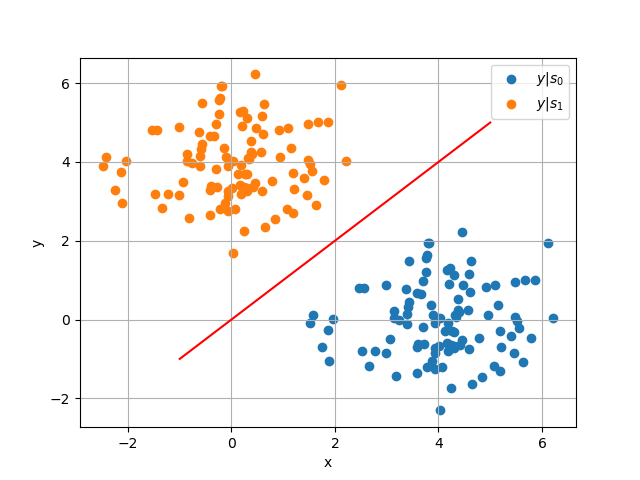
\includegraphics[width=\columnwidth]{./chapters/ch5/figs/ch5_scatter.png}
\caption{Scatter plot of $\mbf{y}|\mbf{s}_0$ and $\mbf{y}|\mbf{s}_1$ }
\label{fig:biv_scatter}
\end{figure}

%
\item
For the above problem, find a decision rule for detecting the symbols $\mbf{s}_0 $ and $\mbf{s}_1$.\\
\solution Let $\mbf{y} = \myvec{y_1&y_2}^T$. Then the decision rule is
\begin{equation}
	y_1 \dec{0}{1} y_2
	\label{eq:biv_fsk_decision}
\end{equation}
$\vec{y}|\vec{s}_i$ is a random vector with each of its components normally distributed. The PDF of $\vec{y}|\vec{s}_i$ is given by,
\begin{equation}
	p_{\vec{y}|\vec{s}_i}\brak{\vec{y}} = \frac{1}{2\pi\sqrt{\mydet{\vec{\Sigma}}}} \exp\brak{-\frac{1}{2}\brak{\vec{y}-\vec{s}_i}^\top \vec{\Sigma}^{-1} \brak{\vec{y}-\vec{s}_i}}
\end{equation}
Where $\vec{\Sigma}$ is the covariance matrix. Substituting $\vec{\Sigma} = \sigma \vec{I}$,
\begin{align}
	p_{\vec{y}|\vec{s}_i}\brak{\vec{y}} &= \frac{1}{2 \pi \sigma} \exp\brak{-\frac{1}{2 \sigma}\brak{\vec{y}-\vec{s}_i}^\top \vec{I} \brak{\vec{y}-\vec{s}_i}}\\
	&= \frac{1}{2 \pi \sigma} \exp\brak{-\frac{1}{2 \sigma}\brak{\vec{y}-\vec{s}_i}^\top \brak{\vec{y}-\vec{s}_i}}
\end{align}
Assuming equiprobable symbols, use MAP rule in \eqref{eq:map_rule} to find optimum decision. Since there are only two possible symbols %
$\vec{s}_0$ and $\vec{s}_1$, the optimal decision criterion is found by equating $p_{\vec{y}|\vec{s}_0}$ and $p_{\vec{y}|\vec{s}_1}$.
\begin{align*}
	p_{\vec{y}|\vec{s}_0} &= p_{\vec{y}|\vec{s}_1}
\end{align*}
	
\begin{multline*}
	\implies \exp\brak{-\frac{1}{2 \sigma}\brak{\vec{y}-\vec{s}_0}^\top \brak{\vec{y}-\vec{s}_0}} = \\
	\exp\brak{-\frac{1}{2 \sigma}\brak{\vec{y}-\vec{s}_1}^\top \brak{\vec{y}-\vec{s}_1}}
\end{multline*}
	
\begin{align*}
	\implies \brak{\vec{y}-\vec{s}_0}^\top \brak{\vec{y}-\vec{s}_0} &= \brak{\vec{y}-\vec{s}_1}^\top \brak{\vec{y}-\vec{s}_1}\\
	\implies \vec{y}^\top\vec{y} - 2\vec{s}_0^\top \vec{y} + \vec{s}_0^T\vec{s}_0 &= \vec{y}^\top\vec{y} - 2\vec{s}_1^\top \vec{y} + \vec{s}_1^T\vec{s}_1\\
	\implies 2\brak{\vec{s}_1-\vec{s}_0}^\top \vec{y} &= \norm{\vec{s}_1}^2 - \norm{\vec{s}_0}^2\\
	\implies \brak{\vec{s}_1-\vec{s}_0}^\top \vec{y} &= 0\\
	\implies \myvec{-1\\1}^\top \vec{y} &= 0
\end{align*}
%
\item
Plot 
\begin{equation} 
P_e = \pr{\hat{\mbf{x}} = \mbf{s}_1|\mbf{x} = \mbf{s}_0}
\label{eq:prob_error_fsk}
\end{equation}
with respect to the SNR from 0 to 10 dB.\\
\solution The blue dots in \figref{fig:biv_pe_snr} are the $P_e$ versus SNR plot. It is generated using the below code,
\begin{lstlisting}
codes/ch5_snr.py
\end{lstlisting}
%
\item
Obtain an expression for $P_e$. Verify this by comparing the theory and simulation plots on the same graph.\\
\solution Using the decision rule from \eqref{eq:biv_fsk_decision},
\begin{align}
	\nonumber
	P_e &= \pr{\hat{\mbf{x}} = \mbf{s}_1|\mbf{x} = \mbf{s}_0}\\\nonumber
	&= \pr{y_1 < y_2|\mbf{x} = \mbf{s}_0}\\\nonumber
	&= \pr{A+n_1 < n_2}\\
	\label{eq:prob_error_fsk_inter}
	&= \pr{n_1-n_2 < -A}
\end{align}
%\textbf{Theorem:} The sum of $N$ independant random variables $X_1,X_2,...,X_N$ with $X_i \sim \gauss{\mu_i}{\sigma_i}$ is itself normally distributed %
%with $\mu =\sum_{i=1}^n \mu_i$ and $\sigma^2 = \sum_{i=1}^n \sigma_i^2$.\\
Let $Z = n_1-n_2$ where $n_1, n_2 \sim \gauss{0}{\sigma^2}$. The PDF of X is given by,
\begin{align}
	\nonumber
	p_Z(z) &= p_{n_1}(n_1) \ast p_{-n_2}(n_2)\\\nonumber
	&= \frac{1}{2\pi\sigma^2}\int_{-\infty}^{\infty} e^{-\frac{t^2}{2\sigma^2}}e^{-\frac{(t-z)^2}{2\sigma^2}}  \,dt\\\nonumber
	&= \frac{1}{2\pi\sigma^2}\int_{-\infty}^{\infty} e^{-\frac{(z-t)^2+t^2}{2\sigma^2}}  \,dt\\\nonumber
	&= \frac{1}{2\pi\sigma^2}\int_{-\infty}^{\infty} e^{-\frac{(2t-z)^2+z^2}{2(\sqrt{2}\sigma)^2}}  \,dt\\\nonumber
	&= \frac{1}{2\pi\sigma^2}e^{-\frac{z^2}{2(\sqrt{2}\sigma)^2}}\int_{-\infty}^{\infty} e^{-\frac{(2t-z)^2}{2(\sqrt{2}\sigma)^2}}  \,dt\\\nonumber
	&= \frac{e^{-\frac{z^2}{2(\sqrt{2}\sigma)^2}}}{\sqrt{2\pi}\sqrt{2}\sigma} \frac{1}{\sqrt{2\pi}\sqrt{2}\sigma}\int_{-\infty}^{\infty} e^{-\frac{k^2}{2(\sqrt{2}\sigma)^2}}  \,dk\\
	\label{eq:std_gauss_diff_pdf_fsk}
	&= \frac{e^{-\frac{z^2}{2(\sqrt{2}\sigma)^2}}}{\sqrt{2\pi}\sqrt{2}\sigma}
\end{align}
From \eqref{eq:std_gauss_diff_pdf_fsk}, $Z \sim \gauss{0}{2\sigma^2}$. Substituting $\sigma=1$, $Z \sim \gauss{0}{2}$. %
\eqref{eq:prob_error_fsk_inter} can be further simplified as,
\begin{align*}
	P_e &= \pr{Z < -A}&\\
	&= \pr{Z > A}&\\
	&= \qfunc{\frac{A}{\sqrt{2}}}&\\
	&= \frac{1}{\sqrt{2\pi}}\int_{\frac{A}{\sqrt{2}}}^{\infty} \exp\left(-\frac{x^2}{2}\right)  \,dx 
\end{align*}
\figref{fig:biv_pe_snr} compares the theoretical and simulation plots.

\begin{figure}[H]
\centering
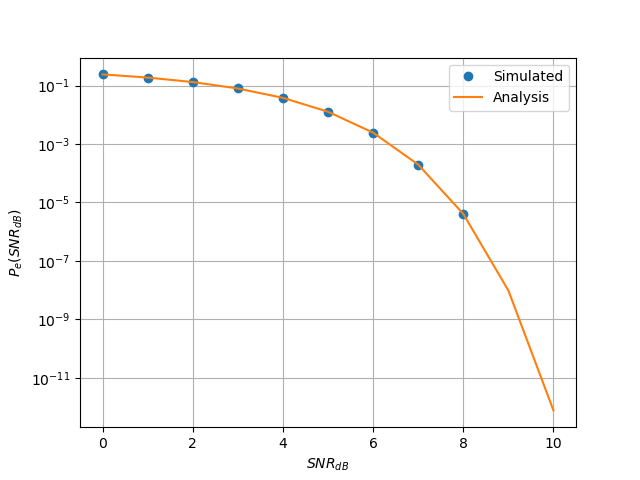
\includegraphics[width=\columnwidth]{./chapters/ch5/figs/ch5_snr.png}
\caption{$P_e$ versus SNR plot for FSK}
\label{fig:biv_pe_snr}
\end{figure}
%
\end{enumerate}

%\end{document}
